
\chapter[Design Flow for Domain-specific Reconfigurable Applications]{Design Flow for Domain-specific Reconfigurable Applications}

\label{ch:tool}

%%%%%%%%%%%%%%%%%%%%%%%%%%%%%%%%%%%%%%%%%%%%%%%%%%%%%%%%%%%%%%%
\section{Introduction}
\label{sec:flow_intro}

In this chapter, we propose a domain-specific design flow for reconfigurable hardware, targeting \gls{smc} in particular.
The main objective of this design flow is to reduce the development effort and optimise the performance of real-time \gls{smc} applications.
Users can specify application-specific features which are automatically converted to efficient hardware so redesign effort is minimised.
A computation engine captures the generic control structure which is shared among all \gls{smc} applications.
All these features are enabled by a framework for mapping software to hardware. 
To enable rapid learning of a large design space, a timing model relates design parameters to performance constraints, and a machine learning algorithm is used to automatically deduce characteristics of the design space.

The contributions are as follows:
\begin{itemize}
\item A design flow that reduces the development effort of \gls{smc} applications on reconfigurable systems (Section~\ref{sec:flow_design}).
The reconfigurable system is generalised based on the one mentioned in Chapter~\ref{ch:adaptation}.
Through templating the \gls{smc} structure, users can design efficient, multiple-\gls{fpga} \gls{smc} applications for arbitrary problems without any knowledge of reconfigurable computing, and the software template is open-source.\footnote{Available online: \url{http://cc.doc.ic.ac.uk/projects/smcgen}}
\item A machine learning approach that explores the \gls{smc} design space automatically and tunes design parameters to improve performance and accuracy (Section~\ref{sec:flow_optimisation}). The resulting parameters can be applied to the hardware design at run-time without the need for resynthesis.
It is demonstrated that parameter optimisation enables the design space to be explored an order of magnitude faster without sacrificing quality.
Compared with previous work~\cite{chau14trets,chau13acm}, we have achieved better quality of solutions and faster designs.
\item The benefit of this approach in terms of design productivity and performance is quantified over a diverse set of \gls{smc} problems.
Three applications are implemented on Altera and Xilinx-based reconfigurable platforms, with varying numbers of \glspl{fpga}. For these problems, the number of lines of code for the \gls{fpga} implementation is reduced by approximately 76\%, and 
significant speedup and energy improvement over \gls{cpu} and \gls{gpu} implementations (Section~\ref{sec:flow_evaluation}) are demonstrated.
\end{itemize}

The rest of the chapter is organised as follows.
Section~\ref{sec:flow_design} describes the design flow for generating reconfigurable \gls{smc} designs.
It covers the software template, the computation engine and the performance model.
Section~\ref{sec:flow_optimisation} discusses how the \gls{smc} computation engine can be optimised both at compile-time and run-time.
Section~\ref{sec:flow_evaluation} evaluates the design flow using 3 different \gls{smc} applications and 
Section~\ref{sec:reconfig_summary} concludes our work.


%%%%%%%%%%%%%%%%%%%%%%%%%%%%%%%%%%%%%%%%%%%%%%%%%%%%%%%%%%%%%%%
\section{SMC Design Flow}
\label{sec:flow_design}

This section introduces a design flow for generating reconfigurable \gls{smc} 
designs. The design flow has two novel features to minimise hardware redesign efforts:
(1) A generic high-level mapping where application-specific features are specified in a software template and automatically converted to hardware.
The template supports the parameter optimisation described in Section~\ref{sec:flow_optimisation}.
(2) A parametrisable \gls{smc} computation engine which is made up of customisable building blocks and generic control structure that maximises design reuse.
We will start with 3 high-level stages as show in Figure~\ref{fig:flow}, and look into the features as we go through this section.
%A novel data structure allows run-time adjustment of parameters.
%These flexibilities minimise hardware redesign efforts and allow \glspl{fpga} to take advantage of the parameter tuning methodology in Section~\ref{sec:optimisation}.

\begin{figure}[ht]
\begin{center}
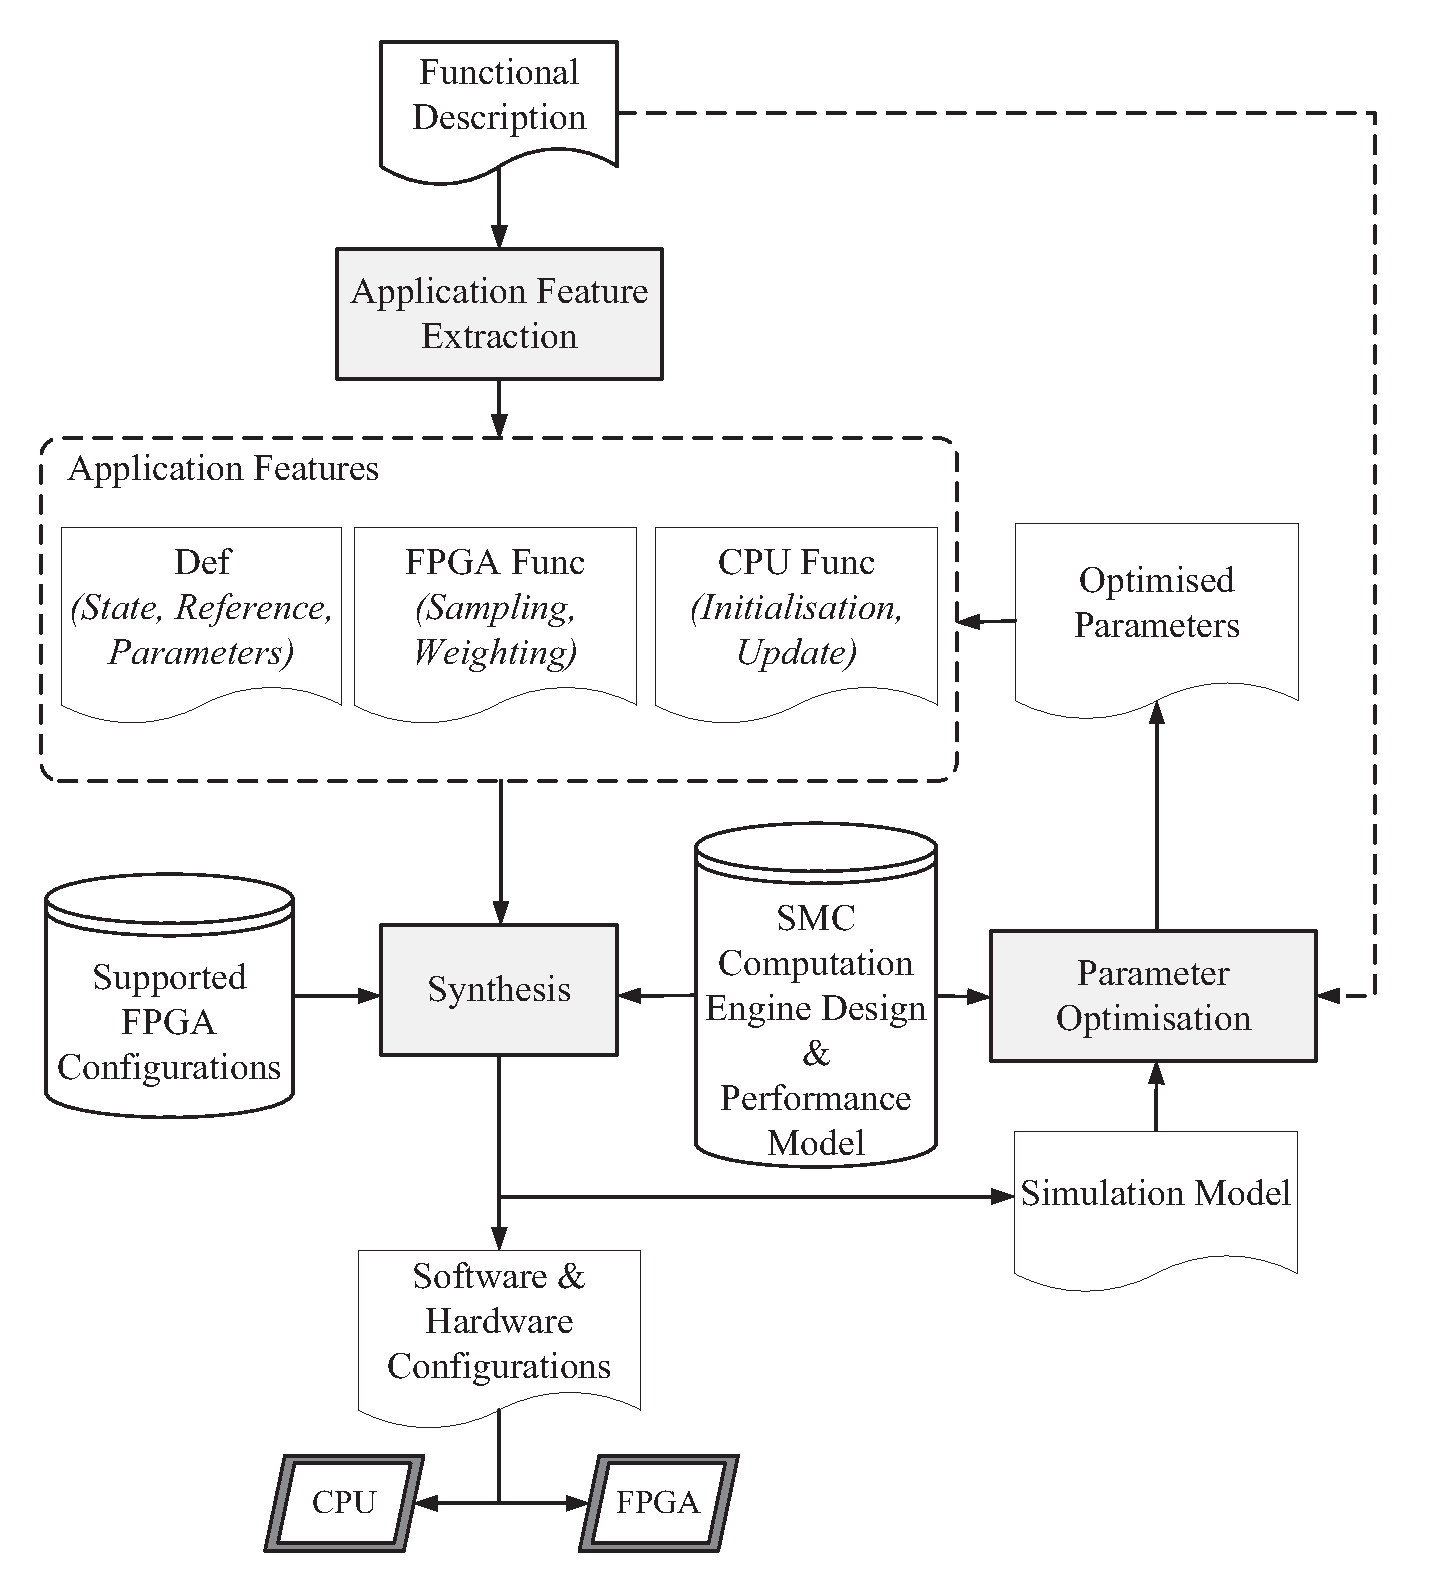
\includegraphics[width=0.8\textwidth]{5_tool/figures/flow}
\end{center}
\caption{Design flow (Compile-time and run-time) for SMC applications. Users only customise the application-specific descriptions inside the dotted box.}
\label{fig:flow}
\end{figure}

Figure~\ref{fig:flow} shows the proposed design flow:

\begin{enumerate}
\item Starting with a functional description such as a software code or a mathematical formulation, the users identify and code application-specific features (Section~\ref{sec:flow_kernel}). 
Generally only the application-specific features are of interest, other features common to all \gls{smc} applications are handled by the design flow, so the functional description does not necessarily have to be a complete software code.

In this work the synthesis tool employed is Maxeler's MaxCompiler, which uses Java as the underlying language. 
MaxCompiler also supports \glspl{fpga} from multiple vendors, such that low level configurations, such as I/O binding, are performed automatically.
Our approach can be extended to support other tools and devices, for example by having the appropriate templates in VHDL or Verilog.
\item The synthesis step automatically weaves the application-specific features with the computation engine (Section~\ref{sec:flow_system}) to form a performance model (Section~\ref{sec:flow_model}), a simulation model, and a complete configuration for the targeted reconfigurable system.
\item The design flow also consists of a parameter optimisation step (Section~\ref{sec:flow_optimisation}) which takes the simulation model and performance model as inputs to produce a set of performance or accuracy optimised parameters.
Generally a simulation model is sufficient for performing optimisation, if a complete software code is provided, it can be used to accelerate the optimisation process.
\item The design of \gls{smc} computation engine allows further adaptation of design at run-time.
The adaptation is based on the solution quality.
For example, a better solution quality means that fewer particles could be used for performing \gls{smc}, and vice versa.
\end{enumerate}




\subsection{Specifying Application Features}
\label{sec:flow_kernel}

Users create a new \gls{smc} design by customising the application-specific Java descriptions inside the dotted box of Figure~\ref{fig:flow}.
These descriptions correspond to \textit{Def} (Code~\ref{lst:def}), \textit{\gls{fpga} Func} (Code~\ref{lst:func}) and \textit{\gls{cpu} Func}.

%\textbf{Def}: Recall from Section~\ref{sec:smc} that \gls{smc} is concerned with estimating state $s_t$ with the effect of control $c_t$. In the example application:
%\textit{state} is location ($x,y$) and heading $h$, and
%\textit{control} is the displacement $d$ and rotation $r$.
%Furthermore, \textit{design parameters} (Table~\ref{tab:parameters}) and application parameters need to be supplied.
\textbf{Def}: Code~\ref{lst:def} illustrates the class where number representation (floating-point, fixed-point with different bit-width), structs (state, reference), static parameters (Table~\ref{tab:parameters}) and system parameters are defined.
Users are allowed to customise number representation to benefit from the flexibility of \gls{fpga} and make trade-off between accuracy and design complexity.
State and reference structs determine the I/O interface.
Static parameters are defined in this class, while dynamic parameters are provided at run-time.
System parameters define device-specific properties such as clock speed and parallelism.
Lastly, application parameters define properties that are tied to specific applications.
%Parameters are mapped to registers or ROMs in the \gls{fpga}.
%For certain applications, the set of parameters can be simplified, e.g.
%\textit{itl\_inner}, \textit{NA} and \textit{H} are set to 1 in this example.

\textbf{\gls{fpga} Func}: \textit{Sampling and importance weighting} (line~\ref{algo:s} and~\ref{algo:i} of Algorithm~\ref{algo:smc}) are the most computation intensive functions, and are accelerated by \glspl{fpga}.
Code~\ref{lst:func} gives a simple example on how these two \gls{fpga} functions are defined.
Given current state \textit{s\_in}, reference \textit{r\_in} and observation \textit{m\_in} (sensor values in this example), an estimation state \textit{s\_out} is computed.
Weight \textit{w} accounts for the probability of an observation from the estimated state.
The weight is calculated from the product of scores over the horizon.
In this example, the weight is equal to the score as the horizon length is only 1. 
%Constraints are then verified, i.e. if any elements of the state vector are negative, the weight is set to zero.

\textbf{\gls{cpu} Func}: \textit{Initialisation and update} are functions running on the \gls{cpu}.
They are responsible for obtaining and formatting data and displaying results.
\textit{Resampling} is independent of applications so users need not to customise it.

\begin{Code}
    \centering
\lstset{language=Java,
        basicstyle=\ttfamily\small,
				tabsize=2,
				numbers=left,
				numberstyle=\tiny,
				frame=tb,
				columns=fullflexible,
				showstringspaces=false
				}
\begin{lstlisting}[][ht]
public class Def {
	// Number Representation
	static final DFEType float_t = 
		KernelLib.dfeFloat(8,24);
	static final DFEType fixed_t = 
		KernelLib.dfeFixOffset(26,-20,SignMode.TWOSCOMPLEMENT);
	// State Struct
	public static final DFEStructType state_t = new 
	DFEStructType(
		new StructFieldType(''x'', float_t);
		new StructFieldType(''y'', float_t);
		new StructFieldType(''h'', float_t););
	// Reference Struct
	public static final DFEStructType ref_t = new 
	DFEStructType(
		new StructFieldType(''d'', float_t);
		new StructFieldType(''r'', float_t););
	// Static Design parameters (Table I)
	public static int NPMin = 5000, NPMax = 25000;
	public static int H = 1, NA = 1;
	// System Parameters
	public static int NC_inner = 1, NC_P = 2;
	public static int Clk_core = 120, Clk_mem = 350;
	public static int FPGA_resampling = 0, Use_DRAM = 0;
	// Application parameters
	public static int NWall = 8, NSensor = 20;
}
\end{lstlisting}
\caption{State, control and parameters for the robot localisation example.}
\label{lst:def}
\end{Code}

\begin{Code}
\centering
\lstset{language=Java,
        basicstyle=\ttfamily\small,
				tabsize=2,
				numbers=left,
				numberstyle=\tiny,
				frame=tb,
				columns=fullflexible,
				showstringspaces=false
				}
\begin{lstlisting}[][ht]
public class Func {
	public static DFEStruct sampling(
		DFEStruct s_in, DFEStruct c_in){
		DFEStruct s_out = state_t.newInstance(this);
		s_out.x = s_in.x + nrand(c_in.d,S*0.5) * cos(s_in.h);
		s_out.y = s_in.y + nrand(c_in.d,S*0.5) * sin(s_in.h);
		s_out.h = s_in.h + nrand(c_in.r,S*0.1);
		return s_out;
	}
	public static DFEVar weighting(
		DFEStruct s_in, DFEVar sensor){
		// Score calculation
		DFEVar score = exp(-1*pow(est(s_in)-sensor,2)/S/0.5);
		// Constraint handling
		bool succeed = est(s_in)>0 ? true : false;
		// Weight accumulation
		DFEVar w = succeed ? score : 0; //weight
		return w;
	}
}
\end{lstlisting}
\caption{FPGA functions (Sampling and importance weighting) for the robot localisation example.}
\label{lst:func}
\end{Code}


\subsection{Computation Engine Design}
\label{sec:flow_system}

In Chapter~\ref{ch:adaptation}, a heterogeneous reconfigurable system has been designed for accelerating \gls{smc} applications.
In this section, the system is extended to improve flexibility in terms of customisability and design friendliness.

To allow customisation of the computation engine, the engine and data structure are designed as shown in Figure~\ref{fig:system} and~\ref{fig:flow_stream} respectively.
The computation engine employs a heterogeneous structure that consists of multiple \glspl{fpga} and \glspl{cpu}.
\glspl{fpga} are responsible for sampling, importance weighting and optionally resampling index generation, and are fully pipelined to maximise throughput. 
To exploit parallelism, particle simulations (sampling and importance weighting) are computed simultaneously by every processing core on each \gls{fpga}. 
Processing cores can be replicated as many times as \gls{fpga} resources allow.
In situation where the computed results have to be grouped together, data are transferred among \glspl{fpga} via an inter-\gls{fpga} connection.
To maximise the system throughput, remaining non-compute-intensive tasks that involve random and non-sequential data accesses are performed on the \glspl{cpu}.
\glspl{fpga} and \glspl{cpu} communicate through high bandwidth connections such as PCI Express or InfiniBand.

\setcounter{subfigure}{0}
\begin{figure}[t!]
\centering
\subfigure[]{
	\includegraphics[width=0.7\textwidth]{5_tool/figures/system}
	\label{fig:system}
}
\subfigure[]{
	\includegraphics[width=0.8\textwidth]{5_tool/figures/stream}
	\label{fig:flow_stream}
}
\caption{(a) Design of the SMC computation engine. Solid lines represent data paths while dotted lines represent control paths; (b) Data structure of particles represented by 3 data streams.}
\end{figure}

From the control paths (dotted lines) of Figure~\ref{fig:system}, we see that there are 3 loops matching Algorithm~\ref{algo:smc}: 
(1) inner, (2) outer, and (3) time step.
First, the inner loop iterates $itl\_inner$ number of times for \textit{sampling} and \textit{importance weighting},
$itl\_inner$ increases with the iteration count of the outer loop.
Second, the outer loop iterates $itl\_outer$ times to do \textit{resampling}.
The resampling process is performed $itl\_outer$ times to refine the pool of particles.
The particle indices are scrambled after this stage and the indices are transferred to the \glspl{cpu} to update the particles.
Third, the time loop iterates once per time step to obtain a new control strategy and update the current state.

Based on this fact, the data structure shown in Figure~\ref{fig:flow_stream} is derived.
%It utilises a deep pipeline of \glspl{fpga} so that particles can be processed simultaneously.
Each particle encapsulates 3 pieces of information: (1) state, (2) reference, and (3) weight, each being stored as a stream as indicated in the figure.
The length of the \textit{state stream} is $N_P \cdot N_A \cdot H$ where $H$ means each control strategy predicts $H$ steps into the future.
The \textit{reference} and \textit{weight streams} have information of $N_A$ agents in $N_P$ particles.

The engine design and data structure do not only offer compile-time parametrisation, in addition, they allow changing the values of $itl\_outer$, $itl\_inner$ and $N_P$ at run-time.
It is because these parameters only affect the length of the particle streams, and not the hardware data path.
The computation engine is fully pipelined and outputs one result per clock cycle.

\begin{figure}[t!]
\begin{center}
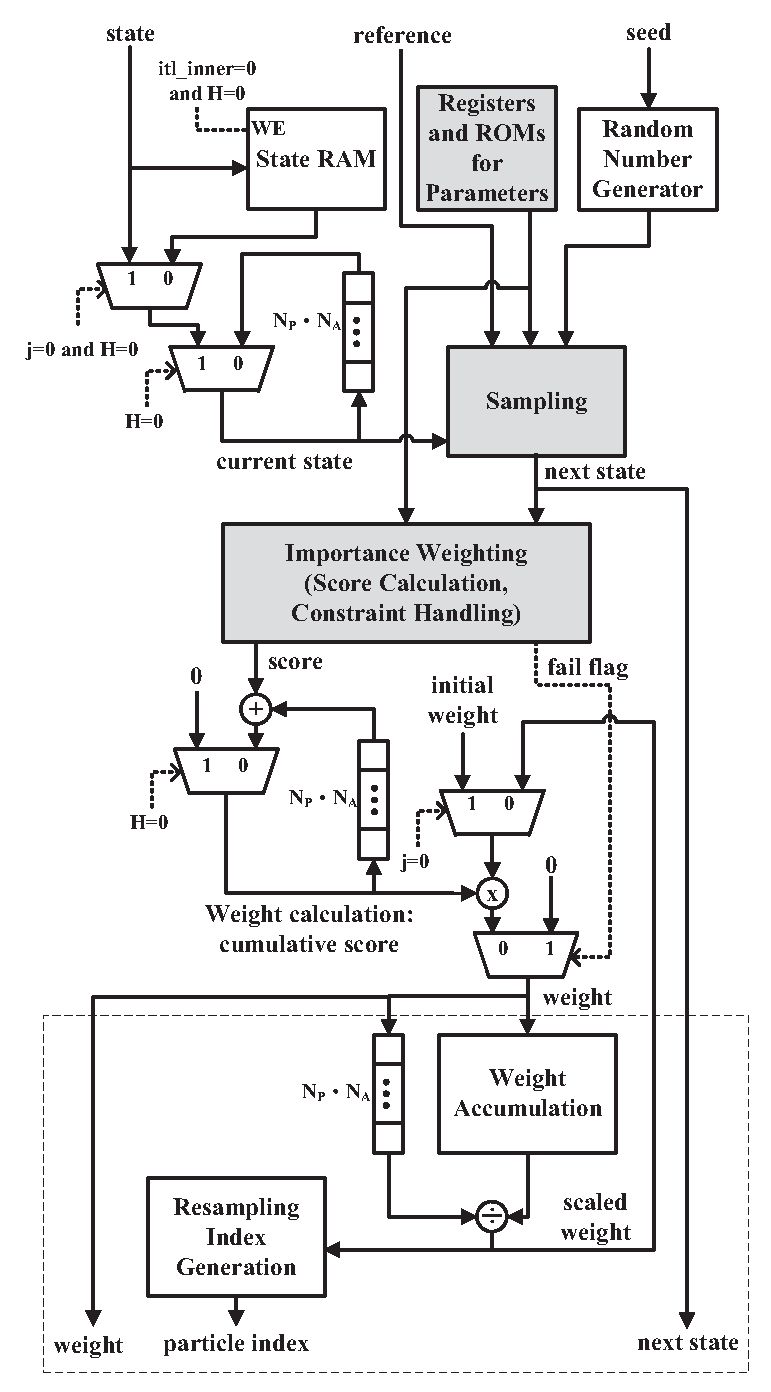
\includegraphics[width=0.6\textwidth]{5_tool/figures/kernel}
\end{center}
\caption{FPGA kernel design. The blocks that require users' customisation are darkened. The dotted box covers the blocks that are optional on FPGAs.}
\label{fig:flow_kernel}
\end{figure}

Figure~\ref{fig:flow_kernel} shows the design of the \gls{fpga} kernel. Blocks that require customisation are darkened.
The sampling function in Code~\ref{lst:func} is mapped to the \textbf{Sampling} block which accepts a state and a reference on each clock cycle and calculates the next state on the prediction horizon.
After getting a state from the \gls{cpu} at the beginning ($itl\_inner=0$ and $H=0$), the data will be used by the kernel $itl\_inner \cdot N_P$ times.
An optional \textit{state RAM} enables reuse of state data and improve performance when the value of $itl\_inner$ is large.
An array of \gls{lut}-based random number generators~\cite{thomas07,thomas10} is seeded by \gls{cpu} to provide random variables; application parameters are stored in registers; and
a feedback path stores the state of the previous $N_P \cdot N_A$ cycles.
%From this value, the next state on the horizon can be computed.

The \textbf{Importance weighting} block computes in 3 steps.
Firstly, \textit{Score calculation} uses the states from the \emph{Next state} block to calculate scores of all the states over the horizon.
A feedback loop of length $N_P \cdot N_A$ stores the cost of the previous horizon and accumulates the values.
Secondly, \textit{Constraint handling} uses the states from the \emph{Next state} block to check the constraints.
The block raises a fail flag if a constraint is violated.
Lastly, \textit{Weight calculation} combines the scores of the states over the horizon.

Part of the resampling process is handled by the \textbf{Resampling index generation} and \textbf{weight accumulation} blocks.
Weights are accumulated to calculate the cumulative distribution function, then particles indices are reordered.
These 2 blocks can either be computed on \glspl{fpga} or \glspl{cpu}.

All the blocks allow precision customisation using fixed-point or floating-point number representation.
Users have the flexibility to make trade-off between result accuracy and design complexity.


\subsection{Performance Model}
\label{sec:flow_model}

We derive a performance model to analyse the effect of parameters on the processing speed and resource utilisation of the computation engine.
It will be used in Section~\ref{sec:flow_optimisation} for parameter optimisation.

The processing time of a time step is shown in Equation~\ref{eqt:time_step}.
It has 4 components which are iterated $itl\_outer$ times.

\begin{equation}
\begin{aligned}
T_{step} = & itl\_outer \cdot \left (T_{s\&i} + T_{resample} + T_{cpu} + T_{transfer} \right)
\end{aligned}
\label{eqt:time_step}
\end{equation}
 
$T_{s\&i}$ is the time spent on sampling and importance weighting in the \gls{fpga} kernels.
Since the data is organised as a stream as described in Section~\ref{sec:flow_system}, the time spent on sampling and importance weighting is linear with $N_P$, $N_A$ and $H$.
It is iterated $itl\_inner$ times in the inner loop.
The sampling and importance weighting process can be accelerated using multiple cores, such that each of them is responsible for part of the inner loop iterations or particles.
$N_C$ represents the number of processing cores being used on one \gls{fpga}, and $N_{Board}$ is the number of \gls{fpga} boards being used.
$min(1,\frac{bandwidth}{sizeof(state) \cdot freq})$ accounts for the limitation of bandwidth between \glspl{fpga} and \glspl{cpu}.

\begin{equation}
\begin{aligned}
T_{s\&i} = \frac{itl\_inner \cdot N_P \cdot N_A \cdot H}{N_C \cdot N_{Board} \cdot freq} \cdot \min\left(1,\frac{bandwidth}{sizeof(state) \cdot freq}\right)
\end{aligned}
\end{equation}

$T_{resample}$ is the time spent on generating the resampling indices.
It takes $N_P \cdot PW + N_P \cdot N_A$ cycles to generate the cumulative probability distribution function, and a further $3 \cdot PL \cdot N_P$ cycles to generate particle indices.
$PW$ and $PL$ are the length of the pipelines.
$T_{resample}$ can be omitted if resampling is processed by the \glspl{cpu}.

\begin{equation}
\begin{aligned}
T_{resample} = \frac{N_P \cdot PW + N_P \cdot N_A + 3 \cdot PL \cdot N_P}{freq}
\end{aligned}
\end{equation}

$T_{cpu}$ is the time spent on resampling and updating the current state on the \glspl{cpu}.
The time is related to the amount of data and the speed of the \gls{cpu}.
$\alpha_1$ is the scaling factor of the \gls{cpu} speed.

\begin{equation}
\begin{aligned}
T_{cpu} = \alpha_1 \cdot H \cdot N_P \cdot N_A
\end{aligned}
\end{equation}

$T_{transfer}$ is the data transfer time that accounts for the time taken to transfer the state stream between \glspl{cpu} and \gls{dram} on an \gls{fpga} board.
$T_{transfer}$ can be omitted if no \gls{dram} is used.

\begin{equation}
\begin{aligned}
T_{transfer} = \frac{N_P \cdot N_A \cdot \left ( H \cdot sizeof(state)\right)}{bandwidth}
\end{aligned}
\end{equation}

%Equation~\ref{eqt:usage_resource} shows the relation of logic, DSP and memory utilisation to parameters.
%$\beta_1, \beta_2, \beta_3, \beta_4, \beta_5$ are application specific parameters.
%The resource utilisations of logic, DSP and memory, denoted as $U_{logic}$, $U_{dsp}$ and $U_{mem}$ respectively, mainly scale with $N_A$.
%The usage of logic and memory is also affected by $N_P$ due to the use of feedback paths.
%$itl\_outer$ and $H$ affect the length of particles streams but not the resource usage.

%\begin{equation}
%\footnotesize
%\begin{aligned}
%U_{logic} & = \beta_1 N_A + \beta_2 N_P \\
%U_{dsp} & = \beta_3 N_A \\
%U_{mem} & = \beta_4 N_A + \beta_5 N_P 
%\end{aligned}
%\label{eqt:usage_resource}
%\end{equation}


%%%%%%%%%%%%%%%%%%%%%%%%%%%%%%%%%%%%%%%%%%%%%%%%%%%%%%%%%%%%%%%
\section{Optimising SMC Computation Engine}
\label{sec:flow_optimisation}

The design parameters in Table~\ref{tab:parameters} have great impact on the performance.
3 questions manifest when finding optimised customisation of the engine:
\textbf{(1) Which sets of parameters have the best accuracy?
(2) For the same accuracy, which sets of parameters meet the timing requirement?
(3) How can we reduce the design parameter exploration time?}
This section discusses some techniques about parameter optimisation.

\subsection{Compile-time Parameters}
\label{sec:flow_parameters}

Referring to Table~\ref{tab:parameters} in Chapter~\ref{ch:background}, the \gls{smc} computation engine has up to 6 design parameters, each of which adds a dimension to the design space.
It is ineffective to exhaustively search for the best set of parameters.
Furthermore, the performance curve of each dimension can be non-linear and constrained by the real-time requirement and \gls{fpga} resources.

To answer \textbf{questions 1 and 2}, consider the robot localisation application.
Its solution quality is measured by \gls{rmse} in localisation.
We study the effect of changing design parameters using the functional specification in Figure~\ref{fig:flow}, e.g. a C program.
Software functional specification has fast build time, and it helps us to perform analysis effectively.
To meet real-time operation requirement, software functional specification is too slow without acceleration of the \gls{smc} computation engine.
The run time of the computation engine is estimated by the timing model described in Section~\ref{sec:flow_model}.

When $N_P$ and $itl\_outer$ are explored together as shown in Figure~\ref{fig:mcl_2d}, we see an uneven surface.
Although non-linear, the trend of  \gls{rmse} decreasing as $N_P$ and $itl\_outer$ are increased is evident.
The valid parameter space is constrained by the real-time requirement:
The parameter space is darkened for those parameters leading to an \gls{rmse} greater than 1 m (Question 1);
The dark region with a run-time longer than the 5 seconds real-time requirement is marked as invalid (Question 2).

\begin{figure}[t!]
\begin{center}
\includegraphics[width=0.8\textwidth]{5_tool/figures/fig_mcl_2d}
\end{center}
\caption{Parameter space of robot localisation system ($N_A$=8192, $S$=1). The dark region on the top-right indicates designs which fail localisation accuracy constraints, while those on the bottom-left indicates designs which fail real-time requirements.}
\label{fig:mcl_2d}
\end{figure}

If the value of $S$ (scaling factor for the standard deviation of noise) is also considered, the parameter optimisation problem expands to 3 dimensions as shown in Equation~\ref{eqt:opt_mcl}.
%In this application, $H=1$ and $itl\_inner=1$ so they are not explored.
%$U_{logic\_A}$, $U_{dsp\_A}$ and $U_{mem\_A}$ denote the resources available on the \gls{fpga}.

\begin{equation}
\begin{aligned}
\mbox{minimise } \gls{rmse} &= f(N_P, itl\_outer, S) \\
\mbox{subject to } \gls{rmse} & \leq \mbox{1 m, } T_{step} \leq \mbox{5s, } \\
%U_{logic} \leq U_{logic\_A} \mbox{, } U_{dsp} & \leq U_{dsp\_A} \mbox{, } U_{mem} \leq U_{mem\_A} \\
\end{aligned}
\label{eqt:opt_mcl}
\end{equation}

%Next we look into \textbf{question 2}, minimising the run time so the robot can move more frequently.
%Although many sets of parameters produce the same solution quality, each set of parameters leads to very different run-time.
%The impact of the real-time constraint emerges in the dark region around the bottom left corner.
%It indicates that some parameter sets lead to designs with run-time exceeding the real-time requirement.

\subsection{Run-time Parameters}

In Chapter~\ref{ch:adaptation}, we proposed an algorithm which changes the number of particles based on run-time condition.
The computation workload decreases with the number of particles and hence introduces an idle period between the finishing time of computation and the end of real-time interval.
The power consumption during the idle period is reduced by reconfigurating the \glspl{fpga} to low-power mode, where the \glspl{fpga} runs at a lower frequency and all the unnecessary features are disabled or removed.
The run-time reconfiguration and parameter adaptation are applied to the proposed \gls{smc} computation engine in this chapter.
For convenience, Algorithm~\ref{algo:smcb} recaptures the approach, with modifications made to cope with the generalised computation engine.
In particular, an inner loop $itl\_inner$ is included to deal with multiple iteration of sampling and importance within a time step.

\begin{algorithm}
\caption{Adaptive SMC algorithm}
{\fontsize{10}{10}\selectfont
\begin{algorithmic}[1]
\STATE{$P_0 \gets P_{max}$}
\STATE{$\{X^{(i)}_0\}^{P_0}_{i=1} \gets $random set of particles}
\STATE{$t \gets 1$}
\FOR{each step $t$}
	\STATE{$idx1 \gets 0$}
	\STATE{Initialisation}
	\WHILE{$idx1 \leq itl\_outer$}
		\STATE{$idx2 \gets 0$}
		\STATE{$itl\_inner \gets f(idx1)$}
		{\color{gray} \STATE{---On \gls{fpga}s---}}
		\WHILE{$idx2 \leq itl\_inner$}
			\STATE{Sample a new state $\{\widetilde{\chi}_{t+1}^{(i)}\}^{P_t}_{i=1}$ from $\{\chi_{t}^{(i)}\}^{P_t}_{i=1}$} \label{algo:smc_si1}
			\STATE{Calculate unnormalised importance weights $\{\widetilde{w}^{(i)}\}^{P_t}_{i=1}$ and accumulate the weights as $w_{sum}$} \label{algo:smc_si2}
			\STATE{$idx2 \gets idx2 + 1$}
		\ENDWHILE
		\STATE{Calculate the lower bound of sample size $\widetilde{P}_{t+1}$ by Equation~\ref{eqt:bound2b}} \label{algo:smc_lb}
	{\color{gray} \STATE{---On \gls{cpu}s---}}
	\STATE{Sort $\{\widetilde{\chi}_{t+1}^{(i)}\}^{P_t}_{i=1}$ in descending $\{\widetilde{w}^{(i)}\}^{P_t}_{i=1}$} \label{algo:smc_sort}
	\IF{$\widetilde{P}_{t+1} < P_{t}$} \label{algo:smc_rd1}
		\STATE{$P_{t+1} = max\left(\lceil\widetilde{P}_{t+1}\rceil, P_{t}/2\right)$}
		\STATE{Set $a = 2P_{t+1}-P_{t}$ and $b = P_{t+1}$}
		{\color{gray} \STATE{--Do the following loop in parallel--}}
		\FOR{$i$ in $P_t-P_{t+1}$} \label{algo:smc_loop1s}
			\STATE{$\widetilde{\chi}^{(i)}_{t+1} = \frac{\chi_{t+1}^{(a)} \widetilde{w}^{(a)} + \chi_{t+1}^{(b)} \widetilde{w}^{(b)}}{\widetilde{w}^{(a)} + \widetilde{w}^{(b)}}$}
			\STATE{$\widetilde{w}^{(i)} = \widetilde{w}^{(a)} + \widetilde{w}^{(b)}$}
			\STATE{$a = a+1$ and $b = b-1$}
		\ENDFOR \label{algo:smc_rd2} \label{algo:smc_loop1e}
	\ELSIF{$\widetilde{P}_{t+1} \geq P_{t}$} \label{algo:smc_rd3}
		\STATE{$a=0$ and $b=0$}
		\FOR{$i$ in $P_{t+1}-P_{t}$}
			\IF{$\widetilde{w}^{(a)}<\widetilde{w}^{(a+1)}$ and $a<P_{t+1}$}
				\STATE{$a=a+1$}
			\ENDIF
			\STATE{$\widetilde{\chi}^{(P_{t}+b)}_{t+1} = \widetilde{\chi}^{(a)}_{t+1}/2$}
			\STATE{$\widetilde{\chi}^{(a)}_{t+1} = \widetilde{\chi}^{(a)}_{t+1}/2$}
			\STATE{$\widetilde{w}^{(P_{t}+b)} = \widetilde{w}^{(a)}/2$}
			\STATE{$\widetilde{w}^{(a)} = \widetilde{w}^{(a)}/2$}
			\STATE{$b=b+1$}
		\ENDFOR
	\ENDIF \label{algo:smc_rd4b}
	\STATE {$idx1 \gets idx1+1$}
	\IF {$idx1 \le itl\_inner$}
	\STATE{Resample $\{\widetilde{\chi}^{(i)}_{t+1}\}^{P_t}_{i=1}$ to $\{\chi^{(i)}_{t+1}\}^{P_{t+1}}_{i=1}$} \label{algo:smc_r}
	\ENDIF
	\ENDWHILE
	\STATE{Update}
\ENDFOR
\end{algorithmic}
}
\label{algo:smcb}
\end{algorithm}

\begin{equation}
\begin{aligned}
\widetilde{P}_{t+1} = \sigma^2 \cdot \frac{P_{max}}{Var(\{\widetilde{\chi}_{t+1}^{(i)}\}^{P_t}_{i=1})}
\end{aligned}
\label{eqt:bound2b}
\end{equation}

Figure~\ref{fig:timing2b} illustrates the effect of adapting parameters at run-time.
Power consumption is reduced by reconfiguring the \glspl{fpga} to sleep mode, at the expense of reconfiguration overhead.

\begin{figure}[t!]
\begin{center}
\includegraphics[width=0.7\textwidth]{4_adaptation/figures/fig_timing2}
\end{center}
\caption{Power consumption of the HRS with reconfiguration to low-power mode during idle}
\label{fig:timing2b}
\end{figure}

\subsection{Parameter Optimisation}
\label{sec:flow_dse}

Now we come to \textbf{question 3}, the parameter optimisation problem, which is difficult as construction of an analytical model combining timing and quality of solution is either impossible or very time consuming. 
Furthermore the design space is constrained by multiple accuracy and real-time requirements.
We cannot use a design unless the results are within certain error bound.
The problem is further aggravated by \textit{the curse of dimensionality}.
%We cannot assume that the general \gls{smc} methods parameters have the same impact on all applications which are based on \gls{smc} methods, the impact can be drastically different.
We use an automated design exploration approach which is facilitated by a machine learning algorithm developed in~\cite{kurek14fccm}.
The approach allows the performance impact of different parameters to be determined for any design based on our \gls{smc} computation engine. 
%The approach has 4 steps:
%(1) Identify metrics to be optimised, such as \gls{rmse} and run-time.
%(2) Specify constraints that distinguish valid and invalid solutions.
%(3) Develop timing and resource models for the \gls{fpga} implementation.
%(4) Use the machine learning approach to explore the parameter space automatically.

A surrogate model is employed to enable rapid learning of the valid design space and deal with a large number of parameters.
%Regression of the fitness function is performed over the parameter space.
%An SVM classifier is used to prevent the algorithm from exploring regions of the parameter space which the classifier predicts to be invalid, i.e. they are likely to fail one of the constraints.
The idea is illustrated in Figure~\ref{fig:dse}.
Firstly, a number of randomly sampled designs is evaluated (Figure~\ref{fig:surrogate_sampling}).
Secondly, the results obtained during evaluations are used to build a surrogate model.
The model provides a regression of a fitness function and identifies regions of the parameter space which fail any of the constraints (Figure~\ref{fig:surrogate_regression}).
Thirdly, the surrogate model output is used to calculate the expected improvement (Figure~\ref{fig:surrogate_ei}).
Finally, the exploration converges to the parameter set that is expected to offer the highest improvement.
Parameter sets in the invalid region are disqualified (Figure~\ref{fig:surrogate_move}).

Our \gls{smc} computation engine is made customisable to benefit from this optimisation approach which is also applicable to \glspl{cpu} and \glspl{gpu}. 

\setcounter{subfigure}{0}
\begin{figure}[t!]
\centering
\subfigure[]{
	\includegraphics[width=0.4\textwidth]{5_tool/figures/fig_surrogate_sampling}
	\label{fig:surrogate_sampling}
}
\subfigure[]{
	\includegraphics[width=0.4\textwidth]{5_tool/figures/fig_surrogate_regression}
	\label{fig:surrogate_regression}
}
\subfigure[]{
	\includegraphics[width=0.4\textwidth]{5_tool/figures/fig_surrogate_ei}
	\label{fig:surrogate_ei}
}
\subfigure[]{
	\includegraphics[width=0.4\textwidth]{5_tool/figures/fig_surrogate_move}
	\label{fig:surrogate_move}
}
\caption{Illustration of automatic parameter optimisation: (a) Sampling parameter sets; (b) Building surrogate model; (c) Calculating expected improvement; (d) Moving to the point offering the highest improvement.}
\label{fig:dse}
\end{figure}


%%%%%%%%%%%%%%%%%%%%%%%%%%%%%%%%%%%%%%%%%%%%%%%%%%%%%%%%%%%%%%%
\section{Evaluation}
\label{sec:flow_evaluation}

%{\bf THOMAS - please comment on how the implementations were verified. Also comment on whether the chosen parameters were the same as the optimal ones (which can be found by exhaustive search).}

%3 applications are used to evaluate the design flow.

\subsection{Design Productivity}

We first analyse how the proposed design flow can reduce design effort.
In Table~\ref{tab:loc}, user-customisable code is classified into three parts:
(a) \textit{Def} is the definition of state, reference and parameters.
(b) \textit{\gls{fpga} Func} is the description of sampling and importance weighting functions.
(c) \textit{\gls{cpu} Func} is the initiation, resampling and update part running on \gls{cpu}.
On average, users only need to customise 24\% of the source code. 
Moreover, automatic design space optimisation greatly saves overall design time.
As we will see in the applications below, we are able to choose the optimal set of parameters without conducting an exhaustive search.
%While this is more difficult to quantify, we conservatively estimate the savings to be more than 50\% of the total design effort.

\begin{table}[ht]
	\setlength{\tabcolsep}{3pt}
	\begin{spacing}{1.0}
	\caption{Lines of code for 3 SMC applications under the proposed design flow.}
	\label{tab:loc}
	\centering
	\smallskip
	\begin{threeparttable}
		\begin{tabular}{l|ccc|c|c}
			\hline
									& \multicolumn{3}{ |c| }{Custom code} &  & \\
									\cline{2-4}
									& Def	& \gls{fpga} Func	& \gls{cpu} Func & All code	& Custom \% \\
			\hline
			\hline
			Sto. vol. 	& 31 & 44  & 84 & 1,164 & 13.7 \\
			Robot loc.	& 54 & 143 & 56 & 1,113 & 22.7 \\
			Air traffic	& 45 & 360 & 70 & 1,360 & 35.0 \\
			\hline
		\end{tabular}
	\end{threeparttable}
	\end{spacing}
\end{table}

\subsection{Application 1: Stochastic Volatility}

The stochastic volatility model was described using the flow 
Our design flow is used in targeting a stochastic volatility model to a XIlinx Virtex-6 XC6VSX475T \gls{fpga} at 150 MHz.
Parallel single precision floating-point data paths are used to maximise resource utilisation and hence performance.
Limited by I/O constraints, 16 processing cores are chosen. The resulting design uses 70,674 \glspl{lut} (24\%), 448 \glspl{dsp} (22\%) and 394 block \glspl{ram} (19\%).
The \gls{cpu} is an Intel Core i7 870 quad-core processor clocked at 2.93GHz.

The design space has 2 dimensions, $N_P$ and $S$ (Table~\ref{tab:parameters}).
No real-time constraint is imposed.
Out of 420 sets of design parameters, the machine learning approach evaluates 20 of the candidates, and obtains an
optimal set of parameters $N_P=768, S=1.5$ which minimises the estimation error.

Table~\ref{tab:perf_sv} summarises the performance of \gls{cpu} and reconfigurable systems using the same set of tuned parameters.
Both systems have the same microATX form factor for fair comparison.

\begin{table}[ht]
	\begin{spacing}{1.0}
	\caption{Performance comparison of stochastic volatility.}
	\label{tab:perf_sv}
	\centering
	\smallskip
	\begin{threeparttable}
		\begin{tabular}{l|x{2.2cm}x{2.2cm}|y{2.2cm}y{2.2cm}}
			\hline
									& \multicolumn{2}{c}{\gls{cpu}~\tnote{a}}	& \multicolumn{2}{c}{This work~\tnote{b}} \\
			\hline
			\hline
			Clock frequency (MHz) 	& \multicolumn{2}{c}{2,930} 				& \multicolumn{2}{c}{150} \\
			Number of cores			& \multicolumn{2}{c}{4}						& \multicolumn{2}{c}{16} \\
			\hline
			\hline
			Number of particles 	& 768	& 76800								& 768  	& 76800 \\
			Run-time per step (ms) 	& 0.05	& 5									& 0.5  	& 0.5 \\
			Power (W)				& 120	& 120								& 140	& 140 \\
			Energy (mJ)				& 6		& 600								& 70 	& 70 \\
			\hline
		\end{tabular}
		\begin{tablenotes}
		\item[a] Intel Core i7 870 \gls{cpu}, optimised by Intel Compiler with SSE4.2 and flag {\it -fast} enabled.
		\item[b] Maxeler MaxWorkstation with Xilinx Virtex-6 XC6VSX475T \gls{fpga} and Intel Core i7 870 \gls{cpu}, developed using MaxCompiler.
		\end{tablenotes}
	\end{threeparttable}
	\end{spacing}
\end{table}

Noted that the data size being processed is very small, therefore the run-time per step is dominated by the overhead of invoking the \gls{fpga} kernels, and initiating the data transfer to \glspl{cpu} and external memory via PCI Express and \gls{dram} controller.
Figure~\ref{fig:est_sv} shows the scenario when larger data sets (more particles) are being used, though in this application using more particles does not justify improvement on the solution quality.
The performance results are estimated using our performance model presented in Section~\ref{sec:flow_model}.
From the figure, it is observed that when the number of particles is larger than 8000, the \gls{smc} computation engine start having performance advantage over \glspl{cpu}.
The run-time of the proposed reconfigurable system is dominated by the overhead when the number of particles is smaller than 2 $\times 10^8$, 
In the next 2 sections, two bigger applications which justify using larger data sets are evaluated.

\begin{figure}[t!]
\centering
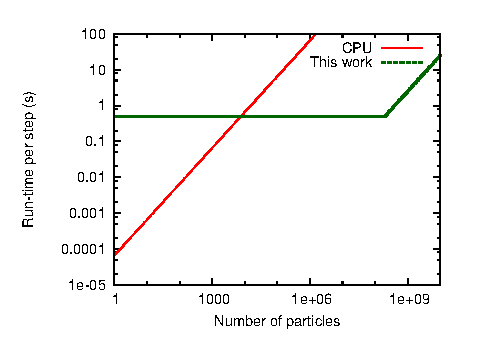
\includegraphics[width=0.7\textwidth]{5_tool/figures/fig_est_sv}
\caption{Stochastic volatility: run-time per step versus data set size}
\label{fig:est_sv}
\end{figure}

\subsection{Application 2: Mobile Robot Localisation}

Now we look at an application with larger data set.
For this example the same reconfigurable system as application 1 is used. 
Two processing cores are instantiated in an \gls{fpga}.
Core computation in the sampling and importance weighting process is implemented using fixed-point arithmetic to optimise resource usage.
The result utilises 148,431 \glspl{lut} (50\%), 1,278 \glspl{dsp} (63\%) and 549 block \glspl{ram} (26\%).

The design space has 3 dimensions: $itl\_outer$, $N_P$ and $S$.
Out of 945 sets of parameters, 52 sets are evaluated to minimise the localisation error within the 5 seconds real-time constraint.

Table~\ref{tab:perf_mcl1} compares the performance of our reconfigurable system with \gls{cpu}, \gls{gpu} and a previous system in~\cite{chau14trets} 
which has not been optimised by our proposed approach.
%The reconfigurable system is 8.9 times and 1.2 times faster than the \gls{cpu} and \gls{gpu}, respectively.
With parameter tuning that maximise accuracy, our work achieves a better \gls{rmse} than the previous work (0.15m vs. 0.52m).
In other words, parameter tuning improves accuracy by 3.5 times.
%It is also the most energy efficient of all systems.
GPU is also optimised using the same set of parameters, but it consumes double the power of our reconfigurable system.
Comparing with CPU, FPGA is 24 times more accurate.
It is because CPU has lower performance, and a different set of parameters is applied to meet the 5 seconds real-time requirement at an expense of accuracy.

\begin{table}[ht]
	\setlength{\tabcolsep}{2pt}
	\begin{spacing}{1.0}
	\caption{Performance comparison of robot localisation.}
	\label{tab:perf_mcl1}
	\centering
	\smallskip
	\begin{threeparttable}
		\begin{tabular}{l|x{3cm}y{3cm}x{3cm}x{3cm}}
			\hline
															& \gls{cpu} 							& This work  				& Ref. sys.~\cite{chau14trets}  	& \gls{gpu} \\
															& opt.~\tnote{a}		&	opt.~\tnote{b}		& w/o opt.~\tnote{b}		& opt. ~\tnote{c} \\
			\hline
			\hline
			Clk. freq. (MHz) 	& 2,930 & 120 	& 100 	& 1,150 \\
			Number of cores					& 4		& 2 	& 2 	& 448 \\
			\hline
			\hline
			Run-time / step (s) 	& 5.0	& 3.7	& 1.6			& 4.5 \\
			\gls{rmse} (m)								& 3.64	& 0.15	& 0.52	& 0.15 \\
			Power (W)								& 130		& 145 	& 145		& 287 \\
			\hline
		\end{tabular}
		\begin{tablenotes}
		\item[a,b] Refer to configurations in Table~\ref{tab:perf_sv}.
		\item[c] NVIDIA Tesla C2070 \gls{gpu}, developed using CUDA programming model.
		\item[d] Parameters with optimisation for FPGA and GPU: $itl\_outer$=2, $N_P$=14000, $S$=1.2; \\ Parameters with optimisation for CPU: $itl\_outer$=1, $N_P$=3000, $S$=1; \\ Parameters without optimisation: $itl\_outer$=1, $N_P$=8192, $S$=1. 
		\end{tablenotes}
	\end{threeparttable}
	\end{spacing}
\end{table}

When parameters of the \gls{smc} computation engine are adapted to the run-time environment, the effect on computation time is shown in Figure~\ref{fig:adaptiveb}.
The largest amount of particles are used to determine the robot's initial location (known as global localisation).
Then the number of particles needed decreases sharply, only a small amount of particles are used to keep tracking the robot's movement.
Reducing in the number of particles implies decrease in the computation time, and hence a longer idle time when the \gls{fpga} runs in low-power mode.

\begin{figure}[t!]
\centering
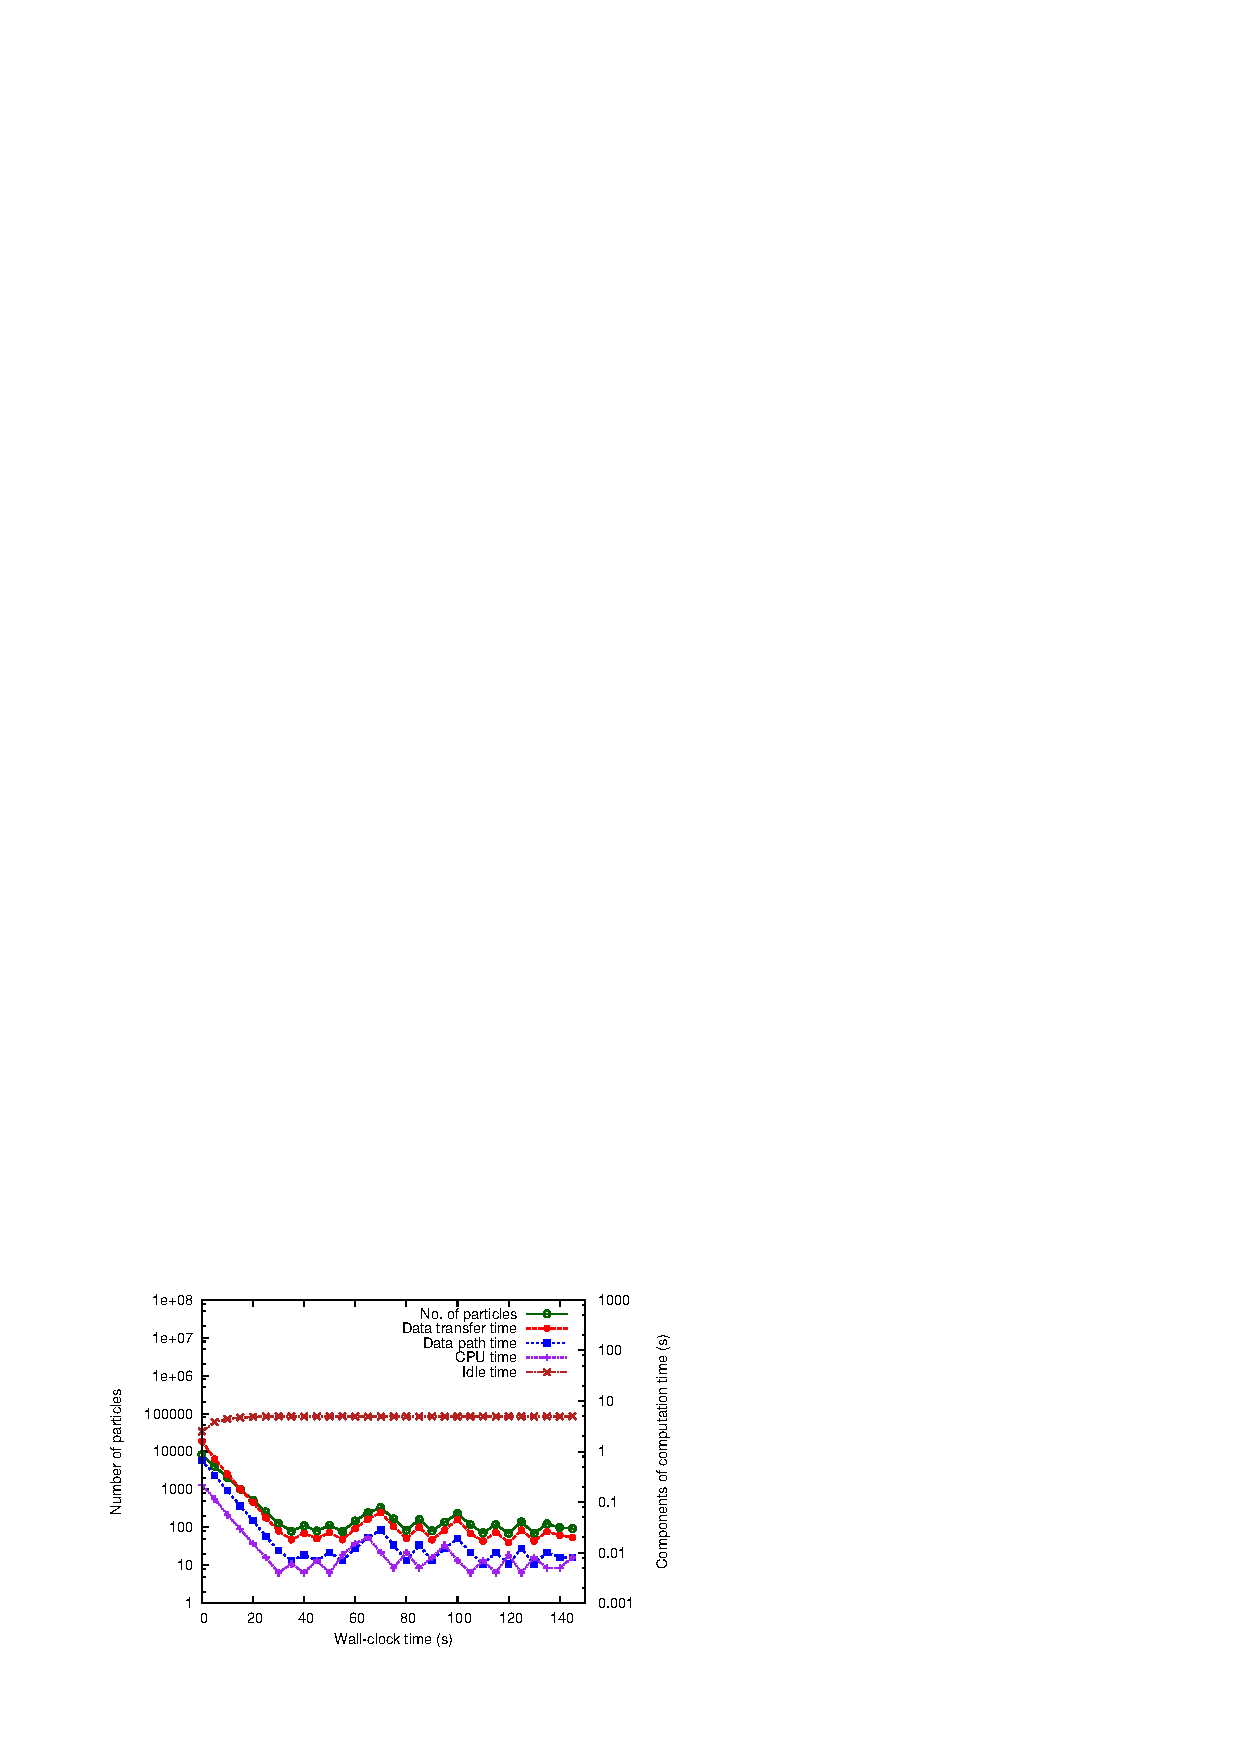
\includegraphics[width=0.7\textwidth]{4_adaptation/figures/fig_adaptive}
\caption{Number of particles and components of total computation time versus wall-clock time}
\label{fig:adaptiveb}
\end{figure}

The effect of running the \gls{fpga} in low-power mode is shown in Figure~\ref{fig:powerb}.
The power of \gls{fpga} peaks at 135W when in compute-mode and drops to 95W when in idle-mode.
Short periods of 110W are observed when the \gls{fpga} is switching between the two modes.
The power of \gls{cpu} and \gls{gpu} are also shown in the figure.
%\todo[inline]{Computation time, run-time, processing-time.}

\begin{figure}[t!]
\centering
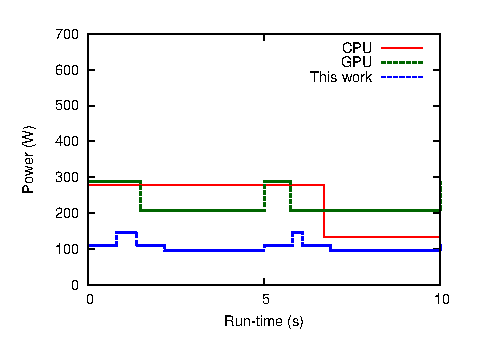
\includegraphics[width=0.7\textwidth]{5_tool/figures/fig_power}
\caption[Power consumption of HRS, CPU and GPU in one time-step, notice that the computation time of the CPU system exceeds the 5-second real-time requirement]{Power consumption of HRS, CPU and GPU in one time-step, notice that the computation time of the CPU system exceeds the 5-second real-time requirement}
\label{fig:powerb}
\end{figure}

\subsection{Application 3: Air Traffic Management}

The air traffic management system is able to control 20 aircraft simultaneously.
The \gls{fpga} part runs on a 1U machine hosting 6 Altera Stratix V GS 5SGSD8 \glspl{fpga} clocked at 220 MHz, 
each of which has a single precision floating-point data path that consumes 166,008 \glspl{lut} (63\%), 337 multipliers (9\%) and 1,528 block \glspl{ram} (60\%).
The \gls{cpu} part runs on 2 Intel Xeon E5-2640 \glspl{cpu} clocked at 2.53GHz.
Both parts are connected via InfiniBand.

This application has 4 design parameters leading to a space with 4000 sets of parameters.
The optimisation target is to minimise the time of aircraft spending in the air traffic control region,
i.e. the number of time steps required for all aircraft to reach their destinations.
Each time step is subject to a real-time requirement of 30 seconds.
Machine learning reduces the number of evaluations to 1\% as indicated in Table~\ref{tab:dse}.
Hence, the parameter optimisation time is reduced from days to hours.

\begin{table}[ht]
	\begin{spacing}{1.0}
	\caption{Parameter optimisation of air traffic management system using machine learning approach.}
	\label{tab:dse}
	\centering
	\smallskip
	\begin{threeparttable}
		\begin{tabular}{l|c|c c c c}
			\hline
			\multirow{2}{*}{$N_A$}			& Parameter	sets		& \multicolumn{4}{|c}{Parameter set obtained} \\
			\cline{3-6}
																	& evaluated / total					& $itl\_outer$  		& $H$ & $N_P$ & $S$ \\
			\hline
			\hline
			4 													& 41 / 4000											& 20								&	5		&	500	  & 0.1 \\
			%12 													& 39 / 4000 											& 20								&	5		&	1000	& 0.05 \\
			20													& 31 / 4000 											& 100								&	8		&	5000	& 0.05 \\
			\hline
		\end{tabular}
	\end{threeparttable}
	\end{spacing}
\end{table}

\begin{table}[ht]
	\setlength{\tabcolsep}{3pt}
	\begin{spacing}{1.0}
	\caption{Performance comparison of air traffic management.}
	\label{tab:perf_comparison}
	\centering
	\smallskip
	\begin{threeparttable}
		\begin{tabular}{c|p{4cm}|ccgc}
			\hline
															&											& \gls{cpu}										& \gls{gpu} 									& This work 					& Ref. \gls{fpga}~\cite{chau13acm} 	\\
															&											& opt.~\tnote{a}		& opt.~\tnote{b} 	& opt.~\tnote{c} & w/o opt.~\tnote{d} 	\\
			\hline
			\hline
															& Clk. freq. (MHz) & 2,660 							& 1,150 								& 220 								& 150  \\
															& Number of cores			& 24										& 1,792									& 6										& 5 \\
															& Power (W)						& 550										& 1100									& 600									& N/A \\
			\hline
			\hline
			4												& Run-time / step (s)	& 0.80		 			&	0.12									&	0.03								& 2.2 \\
			aircraft										& Total steps					& 25						& 25									& 25								& 25 \\
			\hline
			20											& Run-time / step (s)	& Failed	 					&	28.25									&	11.6								& N/A \\
			aircraft										& Total steps					& Failed						& 41									& 41								& N/A \\
			\hline
		\end{tabular}
		\begin{tablenotes}
		\item[a] 4 Intel Xeon X5650 \glspl{cpu} (scaled), optimised by Intel Compiler with SSE4.2 and flag {\it -fast} enabled.
		\item[b] 4 NVIDIA Tesla C2070 \glspl{gpu} (scaled), developed using CUDA programming model.
		\item[c] Maxeler MPC-X2000, with 6 Altera Stratix V GS 5SGSD8 \glspl{fpga} and 2 Intel Xeon X5650 \glspl{cpu}, developed using MaxCompiler.
		\item[d] Altera Stratix IV EP4SGX530 \gls{fpga}.
		\item[e] Parameters with optimisation: refer to Table~\ref{tab:dse};\\ Parameters without optimisation: $itl\_outer$=100, $N_P$=1024, $S$=0.05, $H$=6.
		\end{tablenotes}
	\end{threeparttable}
	\end{spacing}
\end{table}

Table~\ref{tab:perf_comparison} summarises the performance of the \gls{cpu}, \gls{gpu} and reconfigurable system.
To ensure fair comparisons, we scale the \gls{cpu} and \gls{gpu} systems to similar form factors with the reconfigurable system.
The scaling is based on the fact that the sampling and importance weighting process is evenly distributed to every \gls{gpu} and computed independently,
while the resampling process is computed on the \gls{cpu} no matter how many \gls{gpu}s are used.
The reconfigurable platform is faster and more energy efficient than the other systems.

In the case with 4 aircraft, all systems are able to finish with the minimal number of steps without violating the real-time requirement of 30 seconds per step.
However, for the case with 20 aircraft, CPU fails to obtain a parameter set which gives a valid solution within 30 seconds.

We also compare the performance of our work with a reference implementation that uses an Altera Stratix IV \gls{fpga}~\cite{chau13acm}.
That implementation is only large enough to support 4 aircraft and it does not have the flexibility to tune parameters without re-compilation.
Our design exploration approach is able to select the set of parameters that produces the same quality of results and is up to 73 times faster.

%Our \gls{smc} computation engine is also easily scalable.
%For example, in a future scenario with 50 aircraft and a reconfigurable platform with 24 \glspl{fpga}, design exploration indicates that
%we could change the parameter setting to $itl\_outer=120$, $H=10$, $N_P=8000$ and still meet the real-time requirement without any hardware redesign.


%%%%%%%%%%%%%%%%%%%%%%%%%%%%%%%%%%%%%%%%%%%%%%%%%%%%%%%%%%%%%%%
\section{Summary}
\label{sec:flow_summary}

This chapter demonstrates the feasibility of generating highly-optimised reconfigurable designs for \gls{smc} applications, while hiding detailed implementation aspects from the user.  
A software template makes the computation engine portable and facilitates code reuse, the number of lines of user-written code being decreased by approximately 76\% for an application.
We further establish that a surrogate software model combined with machine learning can be used to rapidly optimise designs, reducing optimisation time from days to hours; 
and that the resulting parameters can be utilised without resynthesis. 
%For the stochastic volatility, robot localisation and air traffic management examples explored, the resulting designs improved on the previously best reported implementations.
